\begin{abstract}
Language models produce accurate forecasts, but accuracy alone cannot reveal
whether they reason about how a situation works or rely on surface cues.
Forecasting offers a demanding test: reliable predictions should use relevant
evidence, infer relationships from limited observations, revise them when context
changes, and transfer them beyond familiar cases. Across real forecasting
questions and controlled tasks, models distinguish relevant evidence, adapt to
contextual clues, and benefit from episode-aligned training when mechanisms or
events change. A broad-composition study and the Coin City transfer experiment
extend these tests to unfamiliar synthetic dynamics, while training on historical
markets improves forecasts on held-out events. Together, the results show that
language models infer and reuse predictive structure when a task makes that
structure recoverable.
\end{abstract}

\section{Introduction}
\begin{wrapfigure}{r}{0.52\textwidth}
\vspace{-2.0em}
\centering
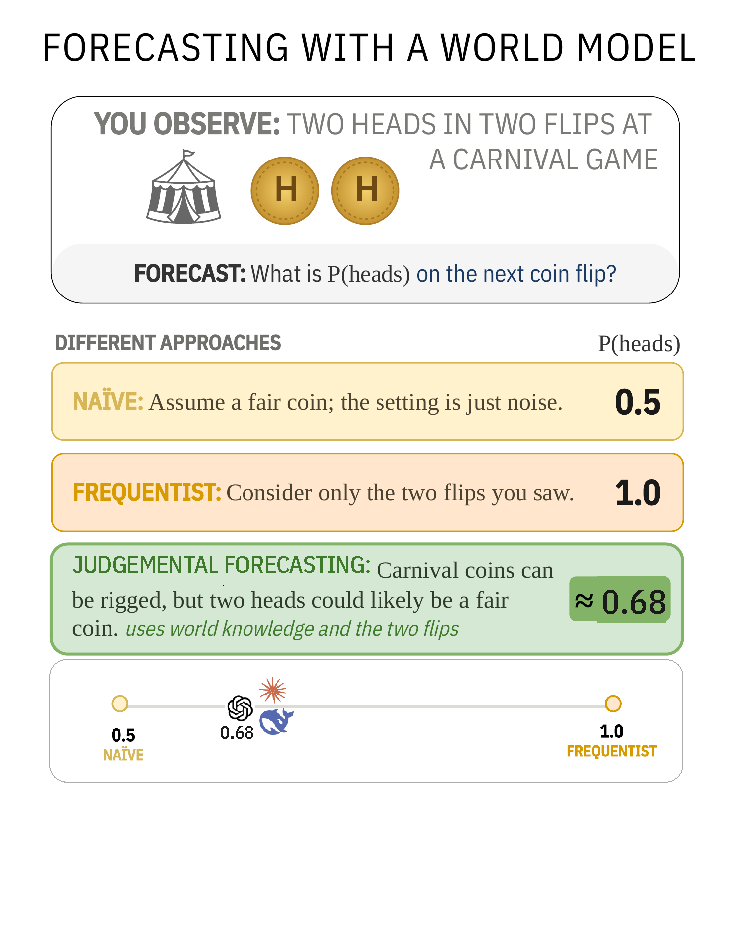
\includegraphics[width=\linewidth,trim=0 72pt 0 0,clip]{figures/teaser_revised.pdf}
\vspace{-0.6cm}
\caption{
\small
After observing two heads in a row at a carnival coin-flipping game, forecasts
differ depending on whether the coin is treated as fair or potentially rigged.
We asked GPT-5.4, Claude Opus~4.8, and DeepSeek V4-Pro to forecast the next-flip
question shown. Each logo marks that model's mean over eight temperature-$0.7$
forecasts: $.644$, $.681$, and $.712$, respectively
(Appendix~\ref{app:carnival-coin-probe}).}
\vspace{-0.5cm}
\label{fig:world-knowledge-evidence}
\end{wrapfigure}

Recent language model (LM) systems approach human-crowd forecasting accuracy, and
model ensembles can match it on some question sets
\citep{halawi2024approaching,schoenegger2024wisdom}. Forecasting agents have now
been tested on Metaculus, Polymarket, and Kalshi, with mixed results
\citep{lu2025evaluating,cao2026auditable,zhang2026prediction}. Their growing ability
motivates our question: \emph{why are language models good at forecasting?}

A forecast connects limited evidence to an outcome through assumptions about how a
process behaves. Figure~\ref{fig:world-knowledge-evidence} illustrates the
distinction: after two heads, the next-flip probability remains $0.5$ if the coin is
known to be fair, but rises when the carnival setting makes a rigged coin plausible.
Real forecasts require similar judgments: whether news matters depends on what it
changes, how long its effect lasts, and how that effect reaches the outcome
\citep{mellers2014psychological,tetlock2016superforecasting}.

The same probability can result from retrieving a similar case, mapping an analogy,
copying a market, or applying a learned model of the process. Prompted rationales
raise accuracy on some reasoning tasks \citep{kojima2022large}, but a verbal
rationale cannot distinguish these possibilities, because generated explanations
need not identify the cause of a model's output
\citep{jacovi2020towards,turpin2023language}.
We therefore ask: \emph{Do language models' forecasts exhibit behavioral signatures
of inductive reasoning over learned world structure?} Here, \textbf{judgemental
forecasting} converts incomplete, heterogeneous evidence into probabilities about
future events. We define \emph{inductive reasoning} as inferring a predictive
relationship from context and observations,
revising that relationship with evidence, and applying it to a new case
\citep{tenenbaum2006theory,tenenbaum2011mind,griffiths2010probabilistic,lake2015human,lake2017building}. \emph{World structure} refers here
to predictive relationships among variables, not to a specified internal
representation.

\subsection{Empirical Approach}
\label{sec:forecasting-as-inductive}

We test three requirements of inductive forecasting:
\begin{itemize}[nosep,leftmargin=*]
  \item \textbf{Selective updating
  (\hyperref[sec:exp1]{Experiment~1}).} On unresolved real questions, we intervene
  on evidence direction and relevance. Across ten models and 38,740 updates,
  forecasts follow the packet's stated direction and move $1.9$--$24\times$ farther
  under directional packets than under topically matched orthogonal ones. The test
  rejects indiscriminate topic reactivity, but a model can pass by classifying the
  packet's stated implication.
  \item \textbf{Context-guided response inference
  (\hyperref[sec:exp2]{Experiment~2}).} In Coin City, matched prompts isolate a
  qualitative cue that links a target city to a response regime. Adding that one
  sentence raises the correlation between forecast-implied and latent
  responsiveness from $-.07$--$.08$ to $\rho=.52$--$.70$ with every number held
  fixed, and inverting it inverts the assignment. Cue inversion and accumulating
  observations reveal whether the model uses and overrides that link; a
  deterministic analogical baseline tests whether explicit mechanism recovery is
  needed.
  \item \textbf{Transfer after training
  (\hyperref[sec:exp3]{Experiments~3 and~4}).} We train forecasting policies and
  extend Coin City by crossing an unseen persistent mechanism with a new surface
  domain. Rewarding episode-specific relationships beats a matched population-prior
  control by $.32$ $[.13,.49]$ MAE under joint domain-and-mechanism shift, and
  training on historical markets lowers sealed-test Brier score from $.1316$ to
  $.1159$ over 1,024 held-out events. A separate appendix study evaluates broader
  unseen mechanism compositions. Matched rewards distinguish episode-specific
  relationships from a population response, while structureless and untrained
  policies diagnose format learning and base-rate improvement.
\end{itemize}

Together, the studies trace forecasting behavior from selective evidence use to
context-guided relationship inference and transfer after training. This sequence
tests whether models reuse predictive relationships rather than evaluating
forecast accuracy alone.

The controls bound what each result establishes. A label-conditioned analogical
regression reproduces the Coin City pattern ($\rho=.66$), episode-aligned training
lowers forecast error without recovering the unseen mediator, and the historical
gain does not exceed contemporaneous market prices. Current models therefore infer
and reuse predictive relationships where the task makes them recoverable; the
controls locate where that ability stops.
